


% Header, overrides base

    % Make sure that the sphinx doc style knows who it inherits from.
    \def\sphinxdocclass{article}

    % Declare the document class
    \documentclass[letterpaper,10pt,english]{/Library/Python/2.7/site-packages/Sphinx-1.2b2-py2.7.egg/sphinx/texinputs/sphinxhowto}

    % Imports
    \usepackage[utf8]{inputenc}
    \DeclareUnicodeCharacter{00A0}{\\nobreakspace}
    \usepackage[T1]{fontenc}
    \usepackage{babel}
    \usepackage{times}
    \usepackage{import}
    \usepackage[Bjarne]{/Library/Python/2.7/site-packages/Sphinx-1.2b2-py2.7.egg/sphinx/texinputs/fncychap}
    \usepackage{longtable}
    \usepackage{/Library/Python/2.7/site-packages/Sphinx-1.2b2-py2.7.egg/sphinx/texinputs/sphinx}
    \usepackage{multirow}

    \usepackage{amsmath}
    \usepackage{amssymb}
    \usepackage{ucs}
    \usepackage{enumerate}

    % Used to make the Input/Output rules follow around the contents.
    \usepackage{needspace}

    % Pygments requirements
    \usepackage{fancyvrb}
    \usepackage{color}
    % ansi colors additions
    \definecolor{darkgreen}{rgb}{.12,.54,.11}
    \definecolor{lightgray}{gray}{.95}
    \definecolor{brown}{rgb}{0.54,0.27,0.07}
    \definecolor{purple}{rgb}{0.5,0.0,0.5}
    \definecolor{darkgray}{gray}{0.25}
    \definecolor{lightred}{rgb}{1.0,0.39,0.28}
    \definecolor{lightgreen}{rgb}{0.48,0.99,0.0}
    \definecolor{lightblue}{rgb}{0.53,0.81,0.92}
    \definecolor{lightpurple}{rgb}{0.87,0.63,0.87}
    \definecolor{lightcyan}{rgb}{0.5,1.0,0.83}

    % Needed to box output/input
    \usepackage{tikz}
        \usetikzlibrary{calc,arrows,shadows}
    \usepackage[framemethod=tikz]{mdframed}

    \usepackage{alltt}

    % Used to load and display graphics
    \usepackage{graphicx}
    \graphicspath{ {figs/} }
    \usepackage[Export]{adjustbox} % To resize

    % used so that images for notebooks which have spaces in the name can still be included
    \usepackage{grffile}


    % For formatting output while also word wrapping.
    \usepackage{listings}
    \lstset{breaklines=true}
    \lstset{basicstyle=\small\ttfamily}
    \def\smaller{\fontsize{9.5pt}{9.5pt}\selectfont}

    %Pygments definitions
    
\makeatletter
\def\PY@reset{\let\PY@it=\relax \let\PY@bf=\relax%
    \let\PY@ul=\relax \let\PY@tc=\relax%
    \let\PY@bc=\relax \let\PY@ff=\relax}
\def\PY@tok#1{\csname PY@tok@#1\endcsname}
\def\PY@toks#1+{\ifx\relax#1\empty\else%
    \PY@tok{#1}\expandafter\PY@toks\fi}
\def\PY@do#1{\PY@bc{\PY@tc{\PY@ul{%
    \PY@it{\PY@bf{\PY@ff{#1}}}}}}}
\def\PY#1#2{\PY@reset\PY@toks#1+\relax+\PY@do{#2}}

\expandafter\def\csname PY@tok@gd\endcsname{\def\PY@tc##1{\textcolor[rgb]{0.63,0.00,0.00}{##1}}}
\expandafter\def\csname PY@tok@gu\endcsname{\let\PY@bf=\textbf\def\PY@tc##1{\textcolor[rgb]{0.50,0.00,0.50}{##1}}}
\expandafter\def\csname PY@tok@gt\endcsname{\def\PY@tc##1{\textcolor[rgb]{0.00,0.27,0.87}{##1}}}
\expandafter\def\csname PY@tok@gs\endcsname{\let\PY@bf=\textbf}
\expandafter\def\csname PY@tok@gr\endcsname{\def\PY@tc##1{\textcolor[rgb]{1.00,0.00,0.00}{##1}}}
\expandafter\def\csname PY@tok@cm\endcsname{\let\PY@it=\textit\def\PY@tc##1{\textcolor[rgb]{0.25,0.50,0.50}{##1}}}
\expandafter\def\csname PY@tok@vg\endcsname{\def\PY@tc##1{\textcolor[rgb]{0.10,0.09,0.49}{##1}}}
\expandafter\def\csname PY@tok@m\endcsname{\def\PY@tc##1{\textcolor[rgb]{0.40,0.40,0.40}{##1}}}
\expandafter\def\csname PY@tok@mh\endcsname{\def\PY@tc##1{\textcolor[rgb]{0.40,0.40,0.40}{##1}}}
\expandafter\def\csname PY@tok@go\endcsname{\def\PY@tc##1{\textcolor[rgb]{0.53,0.53,0.53}{##1}}}
\expandafter\def\csname PY@tok@ge\endcsname{\let\PY@it=\textit}
\expandafter\def\csname PY@tok@vc\endcsname{\def\PY@tc##1{\textcolor[rgb]{0.10,0.09,0.49}{##1}}}
\expandafter\def\csname PY@tok@il\endcsname{\def\PY@tc##1{\textcolor[rgb]{0.40,0.40,0.40}{##1}}}
\expandafter\def\csname PY@tok@cs\endcsname{\let\PY@it=\textit\def\PY@tc##1{\textcolor[rgb]{0.25,0.50,0.50}{##1}}}
\expandafter\def\csname PY@tok@cp\endcsname{\def\PY@tc##1{\textcolor[rgb]{0.74,0.48,0.00}{##1}}}
\expandafter\def\csname PY@tok@gi\endcsname{\def\PY@tc##1{\textcolor[rgb]{0.00,0.63,0.00}{##1}}}
\expandafter\def\csname PY@tok@gh\endcsname{\let\PY@bf=\textbf\def\PY@tc##1{\textcolor[rgb]{0.00,0.00,0.50}{##1}}}
\expandafter\def\csname PY@tok@ni\endcsname{\let\PY@bf=\textbf\def\PY@tc##1{\textcolor[rgb]{0.60,0.60,0.60}{##1}}}
\expandafter\def\csname PY@tok@nl\endcsname{\def\PY@tc##1{\textcolor[rgb]{0.63,0.63,0.00}{##1}}}
\expandafter\def\csname PY@tok@nn\endcsname{\let\PY@bf=\textbf\def\PY@tc##1{\textcolor[rgb]{0.00,0.00,1.00}{##1}}}
\expandafter\def\csname PY@tok@no\endcsname{\def\PY@tc##1{\textcolor[rgb]{0.53,0.00,0.00}{##1}}}
\expandafter\def\csname PY@tok@na\endcsname{\def\PY@tc##1{\textcolor[rgb]{0.49,0.56,0.16}{##1}}}
\expandafter\def\csname PY@tok@nb\endcsname{\def\PY@tc##1{\textcolor[rgb]{0.00,0.50,0.00}{##1}}}
\expandafter\def\csname PY@tok@nc\endcsname{\let\PY@bf=\textbf\def\PY@tc##1{\textcolor[rgb]{0.00,0.00,1.00}{##1}}}
\expandafter\def\csname PY@tok@nd\endcsname{\def\PY@tc##1{\textcolor[rgb]{0.67,0.13,1.00}{##1}}}
\expandafter\def\csname PY@tok@ne\endcsname{\let\PY@bf=\textbf\def\PY@tc##1{\textcolor[rgb]{0.82,0.25,0.23}{##1}}}
\expandafter\def\csname PY@tok@nf\endcsname{\def\PY@tc##1{\textcolor[rgb]{0.00,0.00,1.00}{##1}}}
\expandafter\def\csname PY@tok@si\endcsname{\let\PY@bf=\textbf\def\PY@tc##1{\textcolor[rgb]{0.73,0.40,0.53}{##1}}}
\expandafter\def\csname PY@tok@s2\endcsname{\def\PY@tc##1{\textcolor[rgb]{0.73,0.13,0.13}{##1}}}
\expandafter\def\csname PY@tok@vi\endcsname{\def\PY@tc##1{\textcolor[rgb]{0.10,0.09,0.49}{##1}}}
\expandafter\def\csname PY@tok@nt\endcsname{\let\PY@bf=\textbf\def\PY@tc##1{\textcolor[rgb]{0.00,0.50,0.00}{##1}}}
\expandafter\def\csname PY@tok@nv\endcsname{\def\PY@tc##1{\textcolor[rgb]{0.10,0.09,0.49}{##1}}}
\expandafter\def\csname PY@tok@s1\endcsname{\def\PY@tc##1{\textcolor[rgb]{0.73,0.13,0.13}{##1}}}
\expandafter\def\csname PY@tok@sh\endcsname{\def\PY@tc##1{\textcolor[rgb]{0.73,0.13,0.13}{##1}}}
\expandafter\def\csname PY@tok@sc\endcsname{\def\PY@tc##1{\textcolor[rgb]{0.73,0.13,0.13}{##1}}}
\expandafter\def\csname PY@tok@sx\endcsname{\def\PY@tc##1{\textcolor[rgb]{0.00,0.50,0.00}{##1}}}
\expandafter\def\csname PY@tok@bp\endcsname{\def\PY@tc##1{\textcolor[rgb]{0.00,0.50,0.00}{##1}}}
\expandafter\def\csname PY@tok@c1\endcsname{\let\PY@it=\textit\def\PY@tc##1{\textcolor[rgb]{0.25,0.50,0.50}{##1}}}
\expandafter\def\csname PY@tok@kc\endcsname{\let\PY@bf=\textbf\def\PY@tc##1{\textcolor[rgb]{0.00,0.50,0.00}{##1}}}
\expandafter\def\csname PY@tok@c\endcsname{\let\PY@it=\textit\def\PY@tc##1{\textcolor[rgb]{0.25,0.50,0.50}{##1}}}
\expandafter\def\csname PY@tok@mf\endcsname{\def\PY@tc##1{\textcolor[rgb]{0.40,0.40,0.40}{##1}}}
\expandafter\def\csname PY@tok@err\endcsname{\def\PY@bc##1{\setlength{\fboxsep}{0pt}\fcolorbox[rgb]{1.00,0.00,0.00}{1,1,1}{\strut ##1}}}
\expandafter\def\csname PY@tok@kd\endcsname{\let\PY@bf=\textbf\def\PY@tc##1{\textcolor[rgb]{0.00,0.50,0.00}{##1}}}
\expandafter\def\csname PY@tok@ss\endcsname{\def\PY@tc##1{\textcolor[rgb]{0.10,0.09,0.49}{##1}}}
\expandafter\def\csname PY@tok@sr\endcsname{\def\PY@tc##1{\textcolor[rgb]{0.73,0.40,0.53}{##1}}}
\expandafter\def\csname PY@tok@mo\endcsname{\def\PY@tc##1{\textcolor[rgb]{0.40,0.40,0.40}{##1}}}
\expandafter\def\csname PY@tok@kn\endcsname{\let\PY@bf=\textbf\def\PY@tc##1{\textcolor[rgb]{0.00,0.50,0.00}{##1}}}
\expandafter\def\csname PY@tok@mi\endcsname{\def\PY@tc##1{\textcolor[rgb]{0.40,0.40,0.40}{##1}}}
\expandafter\def\csname PY@tok@gp\endcsname{\let\PY@bf=\textbf\def\PY@tc##1{\textcolor[rgb]{0.00,0.00,0.50}{##1}}}
\expandafter\def\csname PY@tok@o\endcsname{\def\PY@tc##1{\textcolor[rgb]{0.40,0.40,0.40}{##1}}}
\expandafter\def\csname PY@tok@kr\endcsname{\let\PY@bf=\textbf\def\PY@tc##1{\textcolor[rgb]{0.00,0.50,0.00}{##1}}}
\expandafter\def\csname PY@tok@s\endcsname{\def\PY@tc##1{\textcolor[rgb]{0.73,0.13,0.13}{##1}}}
\expandafter\def\csname PY@tok@kp\endcsname{\def\PY@tc##1{\textcolor[rgb]{0.00,0.50,0.00}{##1}}}
\expandafter\def\csname PY@tok@w\endcsname{\def\PY@tc##1{\textcolor[rgb]{0.73,0.73,0.73}{##1}}}
\expandafter\def\csname PY@tok@kt\endcsname{\def\PY@tc##1{\textcolor[rgb]{0.69,0.00,0.25}{##1}}}
\expandafter\def\csname PY@tok@ow\endcsname{\let\PY@bf=\textbf\def\PY@tc##1{\textcolor[rgb]{0.67,0.13,1.00}{##1}}}
\expandafter\def\csname PY@tok@sb\endcsname{\def\PY@tc##1{\textcolor[rgb]{0.73,0.13,0.13}{##1}}}
\expandafter\def\csname PY@tok@k\endcsname{\let\PY@bf=\textbf\def\PY@tc##1{\textcolor[rgb]{0.00,0.50,0.00}{##1}}}
\expandafter\def\csname PY@tok@se\endcsname{\let\PY@bf=\textbf\def\PY@tc##1{\textcolor[rgb]{0.73,0.40,0.13}{##1}}}
\expandafter\def\csname PY@tok@sd\endcsname{\let\PY@it=\textit\def\PY@tc##1{\textcolor[rgb]{0.73,0.13,0.13}{##1}}}

\def\PYZbs{\char`\\}
\def\PYZus{\char`\_}
\def\PYZob{\char`\{}
\def\PYZcb{\char`\}}
\def\PYZca{\char`\^}
\def\PYZam{\char`\&}
\def\PYZlt{\char`\<}
\def\PYZgt{\char`\>}
\def\PYZsh{\char`\#}
\def\PYZpc{\char`\%}
\def\PYZdl{\char`\$}
\def\PYZhy{\char`\-}
\def\PYZsq{\char`\'}
\def\PYZdq{\char`\"}
\def\PYZti{\char`\~}
% for compatibility with earlier versions
\def\PYZat{@}
\def\PYZlb{[}
\def\PYZrb{]}
\makeatother


    %Set pygments styles if needed...
    
        \definecolor{nbframe-border}{rgb}{0.867,0.867,0.867}
        \definecolor{nbframe-bg}{rgb}{0.969,0.969,0.969}
        \definecolor{nbframe-in-prompt}{rgb}{0.0,0.0,0.502}
        \definecolor{nbframe-out-prompt}{rgb}{0.545,0.0,0.0}

        \newenvironment{ColorVerbatim}
        {\begin{mdframed}[%
            roundcorner=1.0pt, %
            backgroundcolor=nbframe-bg, %
            userdefinedwidth=1\linewidth, %
            leftmargin=0.1\linewidth, %
            innerleftmargin=0pt, %
            innerrightmargin=0pt, %
            linecolor=nbframe-border, %
            linewidth=1pt, %
            usetwoside=false, %
            everyline=true, %
            innerlinewidth=3pt, %
            innerlinecolor=nbframe-bg, %
            middlelinewidth=1pt, %
            middlelinecolor=nbframe-bg, %
            outerlinewidth=0.5pt, %
            outerlinecolor=nbframe-border, %
            needspace=0pt
        ]}
        {\end{mdframed}}
        
        \newenvironment{InvisibleVerbatim}
        {\begin{mdframed}[leftmargin=0.1\linewidth,innerleftmargin=3pt,innerrightmargin=3pt, userdefinedwidth=1\linewidth, linewidth=0pt, linecolor=white, usetwoside=false]}
        {\end{mdframed}}

        \renewenvironment{Verbatim}[1][\unskip]
        {\begin{alltt}\smaller}
        {\end{alltt}}
    

    % Help prevent overflowing lines due to urls and other hard-to-break 
    % entities.  This doesn't catch everything...
    \sloppy

    % Document level variables
    \title{StatMech\_HW1}
    \date{February 2, 2014}
    \release{}
    \author{Lei Ma}
    \renewcommand{\releasename}{}

    % TODO: Add option for the user to specify a logo for his/her export.
    \newcommand{\sphinxlogo}{}

    % Make the index page of the document.
    \makeindex

    % Import sphinx document type specifics.
     


% Body

    % Start of the document
    \begin{document}

        
            \maketitle
        

        


        
        

    % Make sure that atleast 4 lines are below the HR
    \needspace{4\baselineskip}

    
        \vspace{6pt}
        \makebox[0.1\linewidth]{\smaller\hfill\tt\color{nbframe-in-prompt}In\hspace{4pt}{[}1{]}:\hspace{4pt}}\\*
        \vspace{-2.65\baselineskip}
        \begin{ColorVerbatim}
            \vspace{-0.7\baselineskip}
            \begin{Verbatim}[commandchars=\\\{\}]
\PY{o}{\PYZpc{}}\PY{k}{pylab} \PY{n}{inline}
\end{Verbatim}

            
                \vspace{-0.2\baselineskip}
            
        \end{ColorVerbatim}
    

    

        % If the first block is an image, minipage the image.  Else
        % request a certain amount of space for the input text.
        \needspace{4\baselineskip}
        
        

            % Add document contents.
            
                \begin{InvisibleVerbatim}
                \vspace{-0.5\baselineskip}
\begin{alltt}Populating the interactive namespace from numpy and matplotlib
\end{alltt}

            \end{InvisibleVerbatim}
            
        
    


    % Make sure that atleast 4 lines are below the HR
    \needspace{4\baselineskip}

    
        \vspace{6pt}
        \makebox[0.1\linewidth]{\smaller\hfill\tt\color{nbframe-in-prompt}In\hspace{4pt}{[}16{]}:\hspace{4pt}}\\*
        \vspace{-2.65\baselineskip}
        \begin{ColorVerbatim}
            \vspace{-0.7\baselineskip}
            \begin{Verbatim}[commandchars=\\\{\}]
\PY{k+kn}{from} \PY{n+nn}{sympy} \PY{k+kn}{import} \PY{o}{*}
\PY{k+kn}{from} \PY{n+nn}{pylab} \PY{k+kn}{import} \PY{o}{*}
\end{Verbatim}

            
                \vspace{-0.2\baselineskip}
            
        \end{ColorVerbatim}
    


    % Make sure that atleast 4 lines are below the HR
    \needspace{4\baselineskip}

    
        \vspace{6pt}
        \makebox[0.1\linewidth]{\smaller\hfill\tt\color{nbframe-in-prompt}In\hspace{4pt}{[}3{]}:\hspace{4pt}}\\*
        \vspace{-2.65\baselineskip}
        \begin{ColorVerbatim}
            \vspace{-0.7\baselineskip}
            \begin{Verbatim}[commandchars=\\\{\}]
\PY{k+kn}{import} \PY{n+nn}{matplotlib.pyplot} \PY{k+kn}{as} \PY{n+nn}{plt}
\end{Verbatim}

            
                \vspace{-0.2\baselineskip}
            
        \end{ColorVerbatim}
    


    % Make sure that atleast 4 lines are below the HR
    \needspace{4\baselineskip}

    
        \vspace{6pt}
        \makebox[0.1\linewidth]{\smaller\hfill\tt\color{nbframe-in-prompt}In\hspace{4pt}{[}4{]}:\hspace{4pt}}\\*
        \vspace{-2.65\baselineskip}
        \begin{ColorVerbatim}
            \vspace{-0.7\baselineskip}
            \begin{Verbatim}[commandchars=\\\{\}]
\PY{k+kn}{from} \PY{n+nn}{sympy.interactive} \PY{k+kn}{import} \PY{n}{printing}
\PY{n}{printing}\PY{o}{.}\PY{n}{init\PYZus{}printing}\PY{p}{(}\PY{n}{use\PYZus{}latex}\PY{o}{=}\PY{n+nb+bp}{True}\PY{p}{)}
\PY{k+kn}{from} \PY{n+nn}{IPython.display} \PY{k+kn}{import} \PY{n}{display}
\PY{n}{a}\PY{p}{,}\PY{n}{x}\PY{p}{,}\PY{n}{Z} \PY{o}{=} \PY{n}{symbols}\PY{p}{(}\PY{l+s}{\PYZsq{}}\PY{l+s}{a,x,Z}\PY{l+s}{\PYZsq{}}\PY{p}{)}
\end{Verbatim}

            
                \vspace{-0.2\baselineskip}
            
        \end{ColorVerbatim}
    
\subsection{Problem 1}\label{problem-1}\subsubsection{1D}\label{d}The partition function for 1D system is$Z = \sum_i e^{-\beta E_i}$The probability on a state $E_i$\[P(E_i) = \frac{e^{-\beta E_i}}{Z}\]In our case, there are only two possible energy states, $E_1 = -\mu B$,
$E_2 = \mu B$. So the magnetization is\[ M =  \mu N \left( e^{\beta \mu B} - e^{-\beta \mu B} \right)/Z\]Write magnetization as a function of $T$ and $T$.\[M(T,B) = \mu N \frac{ \left( e^{\mu B /(k_B T)} - e^{- \mu B/(k_B T)} \right)  }  {  \left(  e^{\mu B /(k_B T)} + e^{- \mu B/(k_B T)}  \right)  } = \mu N \tanh(\mu B /(k_B T))\]$M$ vs $T$ PlotsTo plot $M~T$, we need to make a quantity with dimension of $T$ .
$\bar T = \mu B/k_B$ will do the work.\[\frac{M(T)}{\bar M} = e^{\bar T/T} - e^{-\bar T/T} \]in which, $\bar M = \mu N$ .At $T \rightarrow \infty$ limit, we have the magnetization $M$ is 0.
This is because high temperature distroys the alignment of dipoles.

    % Make sure that atleast 4 lines are below the HR
    \needspace{4\baselineskip}

    
        \vspace{6pt}
        \makebox[0.1\linewidth]{\smaller\hfill\tt\color{nbframe-in-prompt}In\hspace{4pt}{[}5{]}:\hspace{4pt}}\\*
        \vspace{-2.65\baselineskip}
        \begin{ColorVerbatim}
            \vspace{-0.7\baselineskip}
            \begin{Verbatim}[commandchars=\\\{\}]
\PY{n}{tanh}\PY{p}{(}\PY{l+m+mi}{0}\PY{p}{)}
\end{Verbatim}

            
                \vspace{-0.2\baselineskip}
            
        \end{ColorVerbatim}
    

    

        % If the first block is an image, minipage the image.  Else
        % request a certain amount of space for the input text.
        \needspace{4\baselineskip}
        
        

            % Add document contents.
            
                \makebox[0.1\linewidth]{\smaller\hfill\tt\color{nbframe-out-prompt}Out\hspace{4pt}{[}5{]}:\hspace{4pt}}\\*
                \vspace{-2.55\baselineskip}\begin{InvisibleVerbatim}
                \vspace{-0.5\baselineskip}
$$0.0$$
            \end{InvisibleVerbatim}
            
        
    
At $T\rightarrow \infty$, we have $\frac{M}{\bar M}$ 1.

    % Make sure that atleast 4 lines are below the HR
    \needspace{4\baselineskip}

    
        \vspace{6pt}
        \makebox[0.1\linewidth]{\smaller\hfill\tt\color{nbframe-in-prompt}In\hspace{4pt}{[}6{]}:\hspace{4pt}}\\*
        \vspace{-2.65\baselineskip}
        \begin{ColorVerbatim}
            \vspace{-0.7\baselineskip}
            \begin{Verbatim}[commandchars=\\\{\}]
\PY{n}{tanh}\PY{p}{(}\PY{n}{inf}\PY{p}{)}
\end{Verbatim}

            
                \vspace{-0.2\baselineskip}
            
        \end{ColorVerbatim}
    

    

        % If the first block is an image, minipage the image.  Else
        % request a certain amount of space for the input text.
        \needspace{4\baselineskip}
        
        

            % Add document contents.
            
                \makebox[0.1\linewidth]{\smaller\hfill\tt\color{nbframe-out-prompt}Out\hspace{4pt}{[}6{]}:\hspace{4pt}}\\*
                \vspace{-2.55\baselineskip}\begin{InvisibleVerbatim}
                \vspace{-0.5\baselineskip}
$$1.0$$
            \end{InvisibleVerbatim}
            
        
    
At very low temperature, the dipoles have no random motion so all
dipoles aligned together thus $M$ is 1.Now plot out this result.

    % Make sure that atleast 4 lines are below the HR
    \needspace{4\baselineskip}

    
        \vspace{6pt}
        \makebox[0.1\linewidth]{\smaller\hfill\tt\color{nbframe-in-prompt}In\hspace{4pt}{[}7{]}:\hspace{4pt}}\\*
        \vspace{-2.65\baselineskip}
        \begin{ColorVerbatim}
            \vspace{-0.7\baselineskip}
            \begin{Verbatim}[commandchars=\\\{\}]
\PY{n}{t} \PY{o}{=} \PY{n}{linspace}\PY{p}{(}\PY{l+m+mi}{0}\PY{p}{,} \PY{l+m+mi}{100}\PY{p}{,} \PY{l+m+mi}{1000}\PY{p}{)}
\PY{n}{mt} \PY{o}{=} \PY{n}{tanh}\PY{p}{(}\PY{l+m+mi}{1}\PY{o}{/}\PY{n}{t}\PY{p}{)}

\PY{n}{fig11} \PY{o}{=} \PY{n}{plt}\PY{o}{.}\PY{n}{figure}\PY{p}{(}\PY{p}{)}

\PY{n}{axes} \PY{o}{=} \PY{n}{fig11}\PY{o}{.}\PY{n}{add\PYZus{}axes}\PY{p}{(}\PY{p}{[}\PY{l+m+mf}{0.1}\PY{p}{,} \PY{l+m+mf}{0.1}\PY{p}{,} \PY{l+m+mf}{0.8}\PY{p}{,} \PY{l+m+mf}{0.8}\PY{p}{]}\PY{p}{)} \PY{c}{\PYZsh{} left, bottom, width, height (range 0 to 1)}

\PY{n}{axes}\PY{o}{.}\PY{n}{plot}\PY{p}{(}\PY{n}{t}\PY{p}{,} \PY{n}{mt}\PY{p}{,} \PY{l+s}{\PYZsq{}}\PY{l+s}{r}\PY{l+s}{\PYZsq{}}\PY{p}{)}

\PY{n}{axes}\PY{o}{.}\PY{n}{set\PYZus{}xlabel}\PY{p}{(}\PY{l+s}{\PYZsq{}}\PY{l+s}{T bar}\PY{l+s}{\PYZsq{}}\PY{p}{)}
\PY{n}{axes}\PY{o}{.}\PY{n}{set\PYZus{}ylabel}\PY{p}{(}\PY{l+s}{\PYZsq{}}\PY{l+s}{M bar}\PY{l+s}{\PYZsq{}}\PY{p}{)}
\PY{n}{axes}\PY{o}{.}\PY{n}{set\PYZus{}title}\PY{p}{(}\PY{l+s}{\PYZsq{}}\PY{l+s}{M \PYZti{} T}\PY{l+s}{\PYZsq{}}\PY{p}{)}\PY{p}{;}
\end{Verbatim}

            
                \vspace{-0.2\baselineskip}
            
        \end{ColorVerbatim}
    

    

        % If the first block is an image, minipage the image.  Else
        % request a certain amount of space for the input text.
        \needspace{4\baselineskip}
        
        

            % Add document contents.
            
                \begin{InvisibleVerbatim}
                \vspace{-0.5\baselineskip}
\begin{alltt}-c:2: RuntimeWarning: divide by zero encountered in divide
\end{alltt}

            \end{InvisibleVerbatim}
            
                \begin{InvisibleVerbatim}
                \vspace{-0.5\baselineskip}
    \begin{center}
    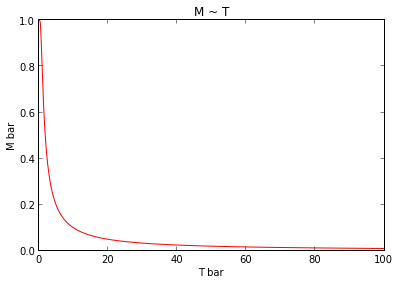
\includegraphics[max size={\textwidth}{\textheight}]{StatMech_HW1_files/StatMech_HW1_24_1.png}
    \par
    \end{center}
    
            \end{InvisibleVerbatim}
            
        
    
This plot agrees with our results of the limits.$M$ vs $B$ PlotsDefine a unit magnetic induction $\bar B = k_B T/\mu$. Write the
magnetization as a function of $B$.\[ \frac{M(B)}{\bar M} = \tanh(B/\bar B) \]At the limit of $B\rightarrow 0$, we have $M\rightarrow 0$, which is
because no magnetic field is there to align the dipoles. (No
interactions between dipoles.)At the limit of $B\rightarrow \infty$, we have $M\rightarrow 1$, which
is because infinite magnetic field can align all the dipoles to one
direction no matter how strong the thermal random motion is.Plot the result.

    % Make sure that atleast 4 lines are below the HR
    \needspace{4\baselineskip}

    
        \vspace{6pt}
        \makebox[0.1\linewidth]{\smaller\hfill\tt\color{nbframe-in-prompt}In\hspace{4pt}{[}8{]}:\hspace{4pt}}\\*
        \vspace{-2.65\baselineskip}
        \begin{ColorVerbatim}
            \vspace{-0.7\baselineskip}
            \begin{Verbatim}[commandchars=\\\{\}]
\PY{n}{b} \PY{o}{=} \PY{n}{linspace}\PY{p}{(}\PY{l+m+mi}{0}\PY{p}{,} \PY{l+m+mi}{5}\PY{p}{,} \PY{l+m+mi}{100}\PY{p}{)}
\PY{n}{mb} \PY{o}{=} \PY{n}{tanh}\PY{p}{(}\PY{n}{b}\PY{p}{)}

\PY{n}{fig12} \PY{o}{=} \PY{n}{plt}\PY{o}{.}\PY{n}{figure}\PY{p}{(}\PY{p}{)}

\PY{n}{axes} \PY{o}{=} \PY{n}{fig12}\PY{o}{.}\PY{n}{add\PYZus{}axes}\PY{p}{(}\PY{p}{[}\PY{l+m+mf}{0.1}\PY{p}{,} \PY{l+m+mf}{0.1}\PY{p}{,} \PY{l+m+mf}{0.8}\PY{p}{,} \PY{l+m+mf}{0.8}\PY{p}{]}\PY{p}{)} \PY{c}{\PYZsh{} left, bottom, width, height (range 0 to 1)}

\PY{n}{axes}\PY{o}{.}\PY{n}{plot}\PY{p}{(}\PY{n}{b}\PY{p}{,} \PY{n}{mb}\PY{p}{,} \PY{l+s}{\PYZsq{}}\PY{l+s}{r}\PY{l+s}{\PYZsq{}}\PY{p}{)}

\PY{n}{axes}\PY{o}{.}\PY{n}{set\PYZus{}xlabel}\PY{p}{(}\PY{l+s}{\PYZsq{}}\PY{l+s}{B/Bbar}\PY{l+s}{\PYZsq{}}\PY{p}{)}
\PY{n}{axes}\PY{o}{.}\PY{n}{set\PYZus{}ylabel}\PY{p}{(}\PY{l+s}{\PYZsq{}}\PY{l+s}{M/Mbar}\PY{l+s}{\PYZsq{}}\PY{p}{)}
\PY{n}{axes}\PY{o}{.}\PY{n}{set\PYZus{}title}\PY{p}{(}\PY{l+s}{\PYZsq{}}\PY{l+s}{M \PYZti{} B}\PY{l+s}{\PYZsq{}}\PY{p}{)}\PY{p}{;}
\end{Verbatim}

            
                \vspace{-0.2\baselineskip}
            
        \end{ColorVerbatim}
    

    

        % If the first block is an image, minipage the image.  Else
        % request a certain amount of space for the input text.
        \needspace{4\baselineskip}
        
        

            % Add document contents.
            
                \begin{InvisibleVerbatim}
                \vspace{-0.5\baselineskip}
    \begin{center}
    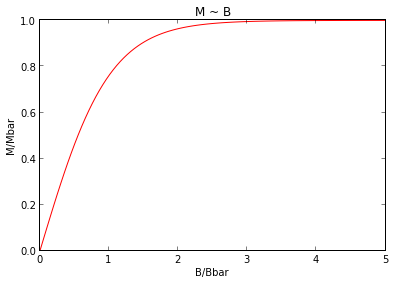
\includegraphics[max size={\textwidth}{\textheight}]{StatMech_HW1_files/StatMech_HW1_32_0.png}
    \par
    \end{center}
    
            \end{InvisibleVerbatim}
            
        
    
Heat CapacityEnergy of the system is\[ E = - \mu B N \tanh(\mu B /(k_B T)) \]

    % Make sure that atleast 4 lines are below the HR
    \needspace{4\baselineskip}

    
        \vspace{6pt}
        \makebox[0.1\linewidth]{\smaller\hfill\tt\color{nbframe-in-prompt}In\hspace{4pt}{[}9{]}:\hspace{4pt}}\\*
        \vspace{-2.65\baselineskip}
        \begin{ColorVerbatim}
            \vspace{-0.7\baselineskip}
            \begin{Verbatim}[commandchars=\\\{\}]
\PY{n}{t13e} \PY{o}{=} \PY{n}{linspace}\PY{p}{(}\PY{l+m+mi}{0}\PY{p}{,} \PY{l+m+mi}{5}\PY{p}{,} \PY{l+m+mi}{100}\PY{p}{)}
\PY{n}{e1} \PY{o}{=} \PY{o}{\PYZhy{}}\PY{n}{tanh}\PY{p}{(}\PY{n}{t13e}\PY{p}{)}

\PY{n}{fig13e} \PY{o}{=} \PY{n}{plt}\PY{o}{.}\PY{n}{figure}\PY{p}{(}\PY{p}{)}

\PY{n}{axes} \PY{o}{=} \PY{n}{fig13e}\PY{o}{.}\PY{n}{add\PYZus{}axes}\PY{p}{(}\PY{p}{[}\PY{l+m+mf}{0.1}\PY{p}{,} \PY{l+m+mf}{0.1}\PY{p}{,} \PY{l+m+mf}{0.8}\PY{p}{,} \PY{l+m+mf}{0.8}\PY{p}{]}\PY{p}{)} \PY{c}{\PYZsh{} left, bottom, width, height (range 0 to 1)}

\PY{n}{axes}\PY{o}{.}\PY{n}{plot}\PY{p}{(}\PY{n}{t13e}\PY{p}{,} \PY{n}{e1}\PY{p}{,} \PY{l+s}{\PYZsq{}}\PY{l+s}{r}\PY{l+s}{\PYZsq{}}\PY{p}{)}

\PY{n}{axes}\PY{o}{.}\PY{n}{set\PYZus{}xlabel}\PY{p}{(}\PY{l+s}{\PYZsq{}}\PY{l+s}{T/Tbar}\PY{l+s}{\PYZsq{}}\PY{p}{)}
\PY{n}{axes}\PY{o}{.}\PY{n}{set\PYZus{}ylabel}\PY{p}{(}\PY{l+s}{\PYZsq{}}\PY{l+s}{E/Ebar}\PY{l+s}{\PYZsq{}}\PY{p}{)}
\PY{n}{axes}\PY{o}{.}\PY{n}{set\PYZus{}title}\PY{p}{(}\PY{l+s}{\PYZsq{}}\PY{l+s}{E \PYZti{} T}\PY{l+s}{\PYZsq{}}\PY{p}{)}\PY{p}{;}
\end{Verbatim}

            
                \vspace{-0.2\baselineskip}
            
        \end{ColorVerbatim}
    

    

        % If the first block is an image, minipage the image.  Else
        % request a certain amount of space for the input text.
        \needspace{4\baselineskip}
        
        

            % Add document contents.
            
                \begin{InvisibleVerbatim}
                \vspace{-0.5\baselineskip}
    \begin{center}
    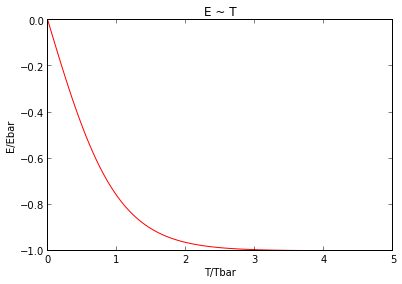
\includegraphics[max size={\textwidth}{\textheight}]{StatMech_HW1_files/StatMech_HW1_36_0.png}
    \par
    \end{center}
    
            \end{InvisibleVerbatim}
            
        
    
Heat capacity is\[ C = \frac{\partial}{\partial T} E = \frac{\mu^2 B^2 N}{k_B} \frac{ (1 - \tanh^2(\mu B/(k_B T)) }{T^2} \]

    % Make sure that atleast 4 lines are below the HR
    \needspace{4\baselineskip}

    
        \vspace{6pt}
        \makebox[0.1\linewidth]{\smaller\hfill\tt\color{nbframe-in-prompt}In\hspace{4pt}{[}10{]}:\hspace{4pt}}\\*
        \vspace{-2.65\baselineskip}
        \begin{ColorVerbatim}
            \vspace{-0.7\baselineskip}
            \begin{Verbatim}[commandchars=\\\{\}]
\PY{n}{t13} \PY{o}{=} \PY{n}{linspace}\PY{p}{(}\PY{l+m+mi}{0}\PY{p}{,} \PY{l+m+mi}{5}\PY{p}{,} \PY{l+m+mi}{100}\PY{p}{)}
\PY{n}{c1} \PY{o}{=} \PY{n}{tanh}\PY{p}{(}\PY{n}{t13}\PY{p}{)}

\PY{n}{fig13} \PY{o}{=} \PY{n}{plt}\PY{o}{.}\PY{n}{figure}\PY{p}{(}\PY{p}{)}

\PY{n}{axes} \PY{o}{=} \PY{n}{fig13}\PY{o}{.}\PY{n}{add\PYZus{}axes}\PY{p}{(}\PY{p}{[}\PY{l+m+mf}{0.1}\PY{p}{,} \PY{l+m+mf}{0.1}\PY{p}{,} \PY{l+m+mf}{0.8}\PY{p}{,} \PY{l+m+mf}{0.8}\PY{p}{]}\PY{p}{)} \PY{c}{\PYZsh{} left, bottom, width, height (range 0 to 1)}

\PY{n}{axes}\PY{o}{.}\PY{n}{plot}\PY{p}{(}\PY{n}{t13}\PY{p}{,} \PY{n}{c1}\PY{p}{,} \PY{l+s}{\PYZsq{}}\PY{l+s}{r}\PY{l+s}{\PYZsq{}}\PY{p}{)}

\PY{n}{axes}\PY{o}{.}\PY{n}{set\PYZus{}xlabel}\PY{p}{(}\PY{l+s}{\PYZsq{}}\PY{l+s}{T/Tbar}\PY{l+s}{\PYZsq{}}\PY{p}{)}
\PY{n}{axes}\PY{o}{.}\PY{n}{set\PYZus{}ylabel}\PY{p}{(}\PY{l+s}{\PYZsq{}}\PY{l+s}{C/Cbar}\PY{l+s}{\PYZsq{}}\PY{p}{)}
\PY{n}{axes}\PY{o}{.}\PY{n}{set\PYZus{}title}\PY{p}{(}\PY{l+s}{\PYZsq{}}\PY{l+s}{C \PYZti{} T}\PY{l+s}{\PYZsq{}}\PY{p}{)}\PY{p}{;}
\end{Verbatim}

            
                \vspace{-0.2\baselineskip}
            
        \end{ColorVerbatim}
    

    

        % If the first block is an image, minipage the image.  Else
        % request a certain amount of space for the input text.
        \needspace{4\baselineskip}
        
        

            % Add document contents.
            
                \begin{InvisibleVerbatim}
                \vspace{-0.5\baselineskip}
    \begin{center}
    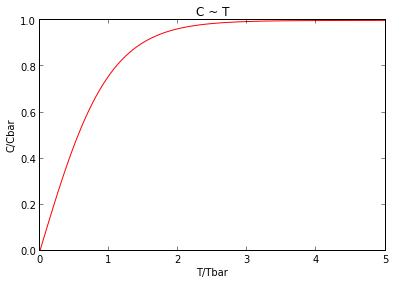
\includegraphics[max size={\textwidth}{\textheight}]{StatMech_HW1_files/StatMech_HW1_39_0.png}
    \par
    \end{center}
    
            \end{InvisibleVerbatim}
            
        
    
\subsubsection{2D}\label{d}The energy of a dipole can be written as
$E(\theta) = -\mu B \cos\theta$, in which $\theta$ is the angle between
the dipole and magnetic field.Partition function is\[ Z = \int _ \theta 2 e^{-\beta E(\theta)} \mathrm d \theta  = 2\pi \mathrm {BesselI}(0, \mu B \beta) \]where $\mathrm{BesselI}$ is the modified Bessel function of the first
kind.Then we can calculate magnetization, which is given by\[ M = \frac{1}{Z}\int _ \theta 2N\mu \cos\theta e^{-\beta E(\theta)} d \theta  \]The result given by Mathematica is (so bad that I can't make sympy to
deal with such integrations.)\[ M = \mu N \frac{ \mathrm{BesselI}(1, B \beta \mu)  }{ \mathrm{BesselI}(0, B \beta \mu) }\]Energy should be\[ E = - \mu B N \frac{ \mathrm{BesselI}(1, B \beta \mu)  }{ \mathrm{BesselI}(0, B \beta \mu) }\]Heat capacity is the derivitive of energy over temperature.\[ C = B^2 \mu^2 N  \frac{-2 \mathrm{BesselI}(0, B \beta \mu)^2 +  \mathrm{BesselI}(0,\mu\beta B)(  \mathrm{BesselI}(0,\mu\beta B) + \mathrm{BesselI}(2,\mu\beta B)   ) }{2 k T^2 \mathrm{BesselI}(0, B \beta \mu)^2} \]Plot out these results using Mathematica.\begin{figure}[htbp]
\centering
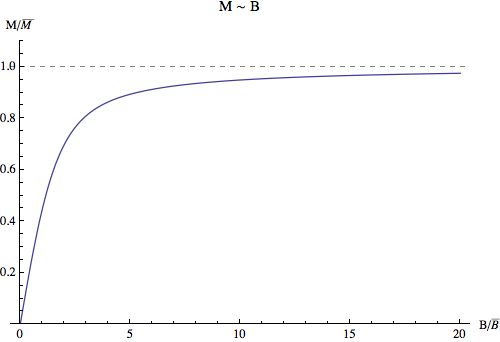
\includegraphics{images/magb2.png}
\end{figure}\begin{figure}[htbp]
\centering
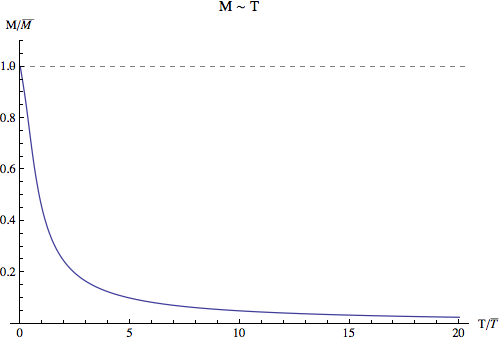
\includegraphics{images/magt2.png}
\end{figure}\begin{figure}[htbp]
\centering
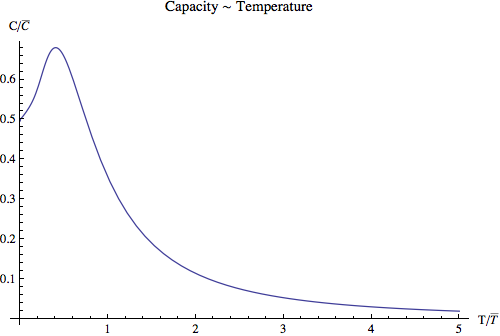
\includegraphics{images/capt2.png}
\end{figure}\subsubsection{3D}\label{d}Energy of a dipole is $E(\theta) = -\mu B \cos\theta$.Then we can calculate the partition function, which is\[ Z = \int_\theta \int _ \phi N e^{-\beta E(\theta)}\sin\theta d\theta d \phi = 4\pi N\frac{ \sinh(\mu B \beta)}{\mu B \beta} \]Magnetization is\[ M =  -\frac{\mu N}{\mu B \beta} + \mu N \coth(\mu B \beta) = \mu N \left(  - \frac{\bar B}{B} + \coth \left(\frac{B}{\bar B}\right) \right) \]where $\bar B = \frac{1}{\mu \beta}$. Define $\bar M = \mu N$ .Then we
can write down the dimensionless equation, which is\[ \frac{M}{\bar M} =  - \frac{\bar B}{B} + \coth \left(\frac{B}{\bar B}\right) \]Total energy is\[ E = \frac{1}{Z} \int _ \phi \int _ \theta (-\mu B \cos\theta N) e^{-\mu E(\theta)}\sin\theta d \theta d\phi = - N \left( \frac{1}{\beta} - B \mu \coth(\mu \beta B) \right)  \]Take the derivative with respect to temperature, we have the heat
capacity.\[ C = N \left( 1 - \left(\frac{\bar T}{T} \right)^2 \mathrm{csch}^2 \left( \frac{\bar T}{T} \right) \right) \]Plot out the results.\begin{figure}[htbp]
\centering
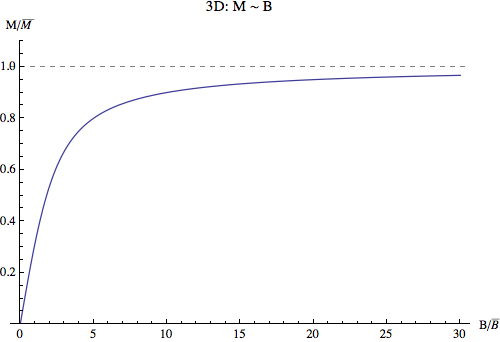
\includegraphics{images/magb3.png}
\end{figure}\begin{figure}[htbp]
\centering
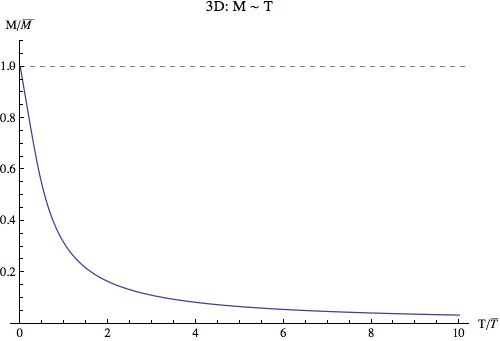
\includegraphics{images/magt3.png}
\end{figure}\begin{figure}[htbp]
\centering
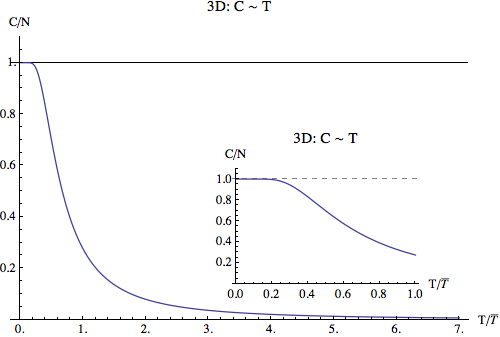
\includegraphics{images/capt3.png}
\end{figure}\subsection{Problem 2}\label{problem-2}\paragraph{First law of
thermodynamics}\label{first-law-of-thermodynamics}Energy can be transfered from one form to another, or from one system to
another, but can never be disapear. The total energy of a closed system
is conserved. For any infinitesimal process, the change of internal
energy is equivalent to the sum of work done to other systems and heat
obsorbed from other systems, which is to say, in the language of
mathematiccs,\subsubsection{\[ \mathrm d U = \mathrm d Q + \mathrm d W \]}\paragraph{Entropy}\label{entropy}Basicly, at high temperature and in large systems, entropy is the
dominant of all marco properties of a system. Entropy indicates the
reversibility of a process, defines Kelvin and restricts us from
reaching absolute zero.The most important property of entropy is that it is a function that
only depends on state of the system not the path. This property can lead
us to many interesting results.\paragraph{Free energy}\label{free-energy}As I have learned in undergrad stat mech, free energy is a quantity
defined to make our life easier when dealing with systems which has
fixed temperature and fixed volume. In that case, free energy can never
grow larger. Mathematically,\[ \mathrm d F \leq 0 \]Suppose we have a gas system going through a reversible process, free
energy\[ \mathrm d F = - S\mathrm d T - p \mathrm d V \]For fixed $T$ and $V$, we have $\mathrm d F = 0$. For irreversible
process, it is less than 0.\paragraph{Chemical potential}\label{chemical-potential}Chemical potential is the increased Gibbs free energy when one mole
particle is added to the system.
        

        \renewcommand{\indexname}{Index}
        \printindex

    % End of document
    \end{document}


